% Chapter 7
\chapter{Experimental results.}\label{Chapter7}
\lhead{Chapter 7. \emph{Experimental Results}}

The final experiment was performed on MOS structures with
inhomogeneous depth profile of the dopant impurities, which was
created by a process ion implantation with different doses in an
N-type silicon single crystal with orientation [100].

Prior to technological processing, the homogeneity was tested of the
specific resistivity of the used silicon wafers by means of a device
Prometrix OmniMap RS35, which uses a four-point method to determine
surface specific resistivity. Table~\ref{tab:7.1} shows the mean
values of the specific resistivity $\overline\rho$ and the standard
deviation of $\delta\rho$ expressed in absolute and relative values.

\begin{table}[h!]\centering
  \begin{tabular}{c c c c c c c c}
    No. & $\overline\rho[\Omega cm]$ & $\delta\rho[\Omega cm]$ & $\delta\rho[\%]$ &
    No. & $\overline\rho[\Omega cm]$ & $\delta\rho[\Omega cm]$ & $\delta\rho[\%]$\\
    \hline% chktex-file 44
    1 & 4.3319 & 0.1223 & 2.822 & 11 & 4.5706 & 0.1658 & 3.627\\
    2 & 4.2733 & 0.1204 & 2.817 & 12 & 4.4762 & 0.1860 & 4.155\\
    3 & 5.1040 & 0.3405 & 6.671 & 13 & 4.3332 & 0.1265 & 2.290\\
    4 & 4.6276 & 0.2080 & 4.494 & 14 & 4.8422 & 0.3573 & 7.380\\
    5 & 4.7697 & 0.1824 & 3.824 & 15 & 4.5917 & 0.1741 & 3.791\\
    6 & 4.8007 & 0.2340 & 4.873 & 16 & 4.8134 & 0.2590 & 5.380\\
    7 & 4.2500 & 0.1436 & 3.378 & 17 & 4.4025 & 0.1527 & 3.468\\
    8 & 4.8259 & 0.3163 & 6.554 & 18 & 4.3591 & 0.1290 & 2.960\\
    9 & 4.2853 & 0.1418 & 3.308 & 19 & 4.3877 & 0.1349 & 3.074\\
    10 & 4.2954 & 0.1113 & 2.592 & 20 & 4.5416 & 0.1618 & 3.563\\
  \end{tabular}
  \caption[Mean and standard deviation of specific resistance of the
    tested silicon wafers before technological processing]{Mean value
    and standard deviation of the specific resistance of the tested
    silicon wafers before technological processing.}\label{tab:7.1}
\end{table}

The Prometrix OmniMap RS35 device measured the the specific resistance
value at 81 points on each plate. At Figure~\ref{fig:7.1} and
Figure~\ref{fig:7.2} we present graphical representation of the
specific resistance distribution, which is also the output of of the
measurement of the above device. The points at which the specific
resistance are indicated in Figure~\ref{fig:7.1} by $+$ or $-$
depending on whether the value of the specific resistance at that
point lay above, or below the mean value, which is shown by the
thicker line.  An idea of the quantitative distribution of the
specific resistance can be can be obtained from the three-dimensional
figure~\ref{fig:7.2}.

The sequence of the main technological operations for the formation of
MOS structures on the substrates mentioned above was as follows

\begin{itemize}
\item formation of a $100 \nu m$ thick gate oxide
\item implantation of $P^{31}$ with energy $120 keV$ and doses 0.6,
  1.0, 2.0, 4.0, 5.0, 6.0, 7.0, 8.0, 20.0, 60.0 $\times 10^{15}
  m^{-2}$ under angle $7\degree$
\item activation at temperature $1050 \degree C$ with time course: 15
  min.\ start-up, 30 min.\ activation, 40 min.\ cooling
\item Al vaporization on both sides of the silicon wafer
\item lithography process to create CV mask
\item sintering of Al FG at $460 \degree C$ for 20 min.
\end{itemize}

20 silicon wafers with a diameter of 4 inches, two each time with the
same implantation dose. In the process of data collection 304
structures were tested on each silicon wafer, with the area of one
structure was $0.81 \times 10^{-6} m^{-2}$. At Figure~\ref{fig:7.3}
shows the concentration profiles of the dopants for each implantation
dose. Shown waveforms represent the mean over all $N(x)$ dependencies,
that have been determined on the test plate. From each batch, the
Figure~\ref{fig:7.3} only one silicon wafer is shown.

\newpage
\begin{figure}[h!]\centering
  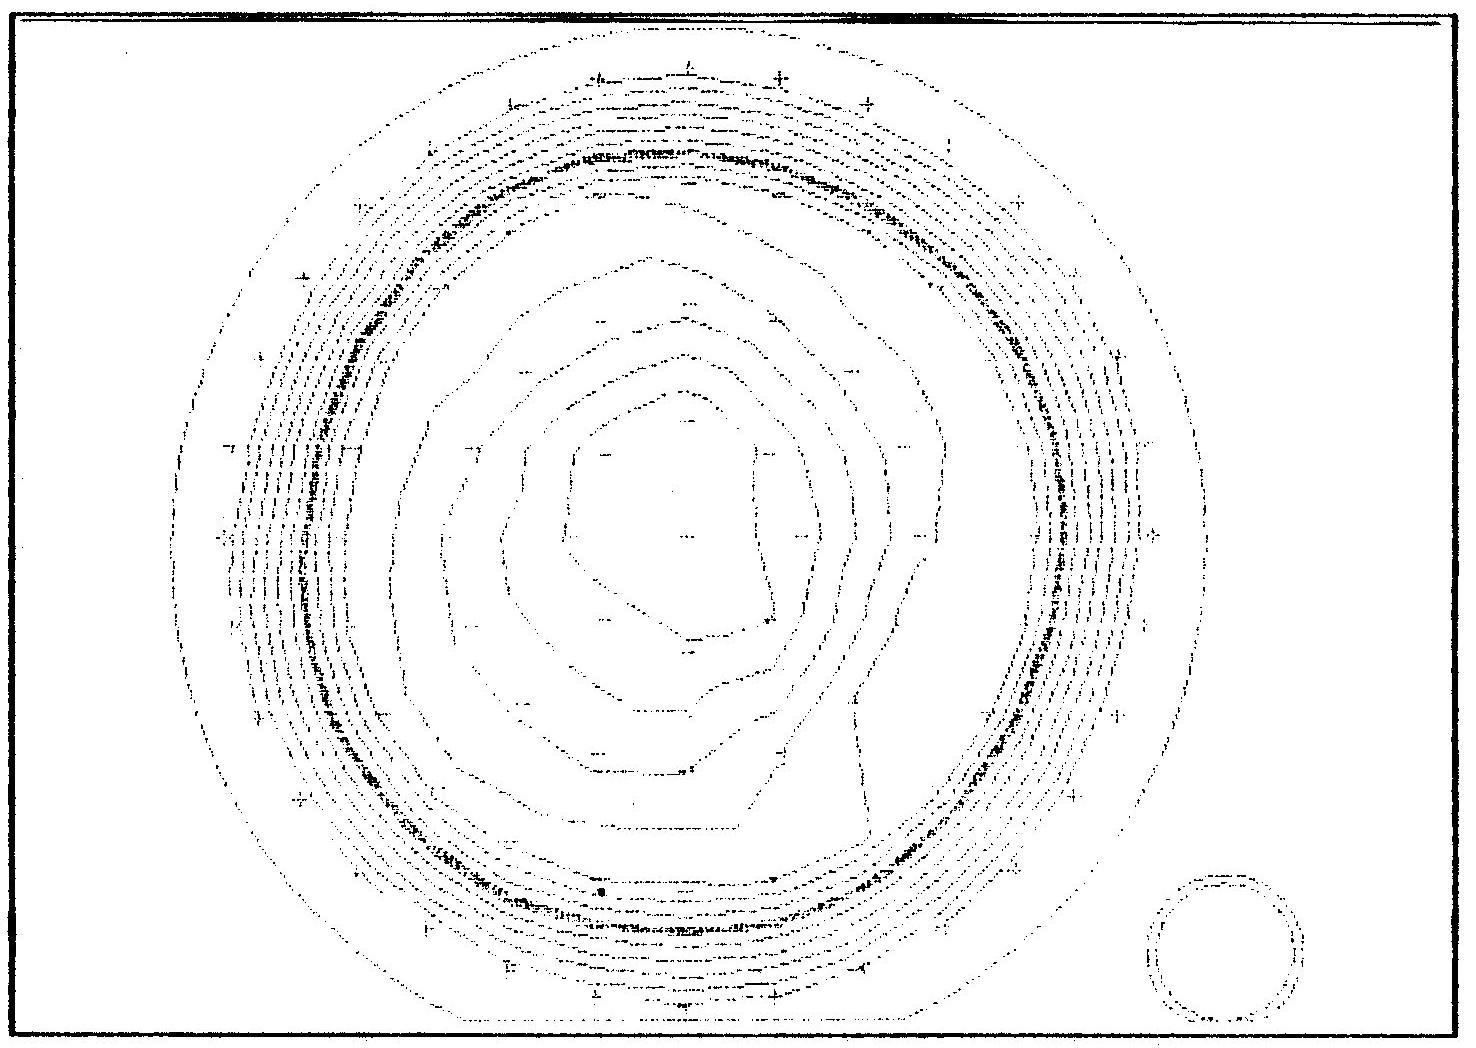
\includegraphics{Figures/fig-7-1.eps}% chktex-file 8
  \caption[Area distribution of surface specific resistance of silicon
    wafer No.16]{Surface Specific Resistivity Distribution specific
    resistivity of silicon wafer No.16.}\label{fig:7.1}
\end{figure}

\begin{figure}[h!]\centering
  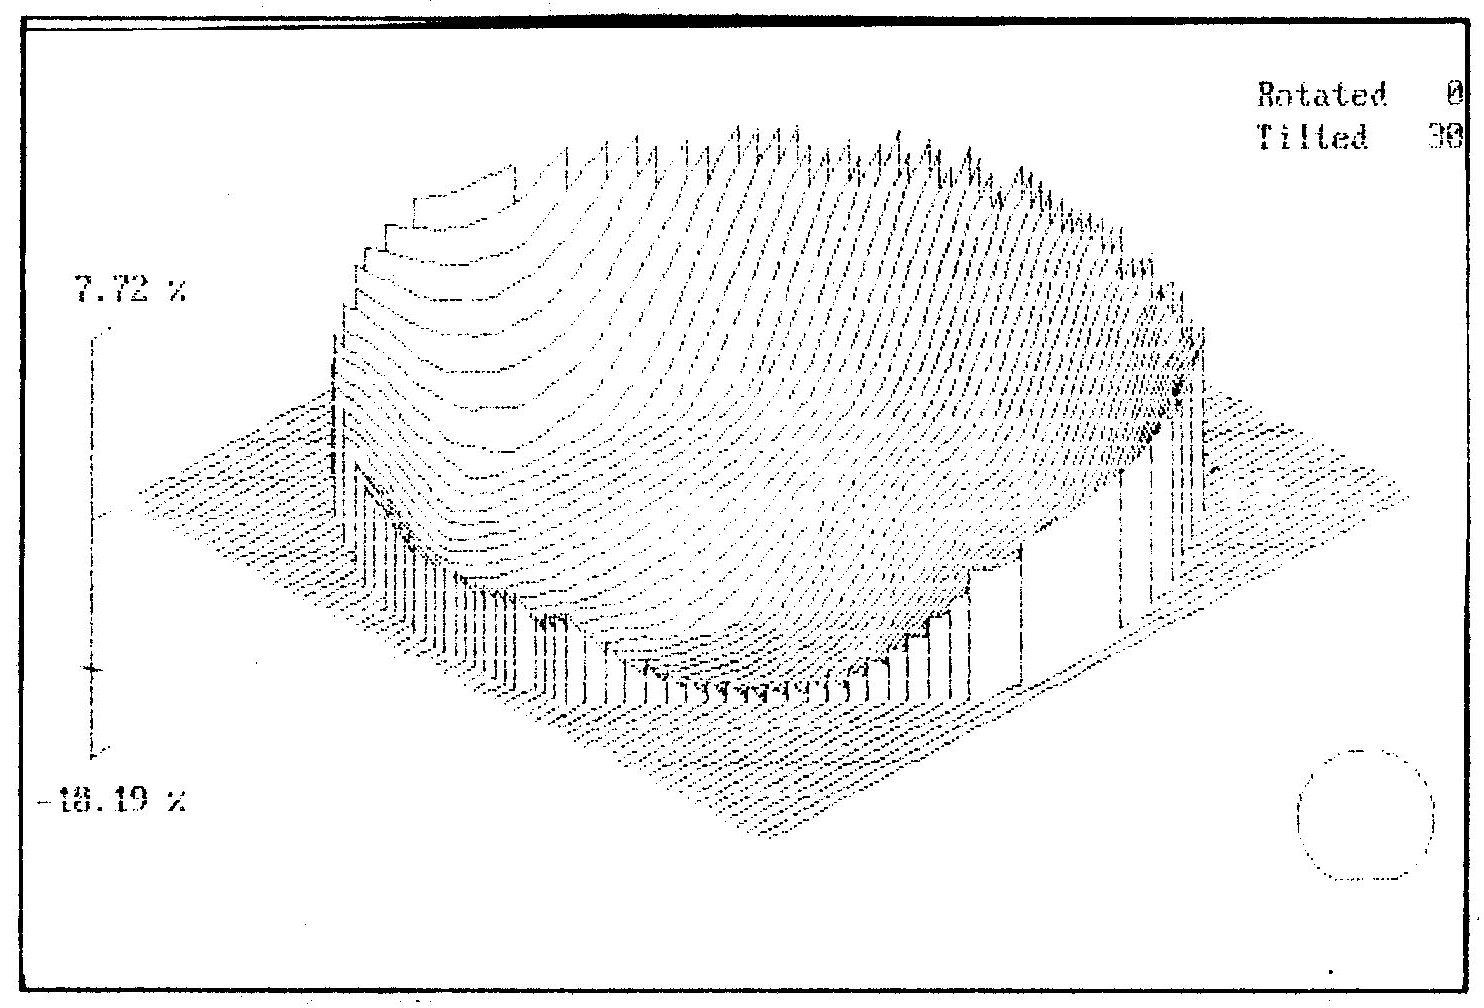
\includegraphics{Figures/fig-7-2.eps}
  \caption[Area distribution of surface specific resistance of silicon
    wafer No.16]{Surface Specific Resistivity Distribution of silicon
    wafer No.16.}\label{fig:7.2}
\end{figure}

\newpage
\begin{figure}[h!]\centering
  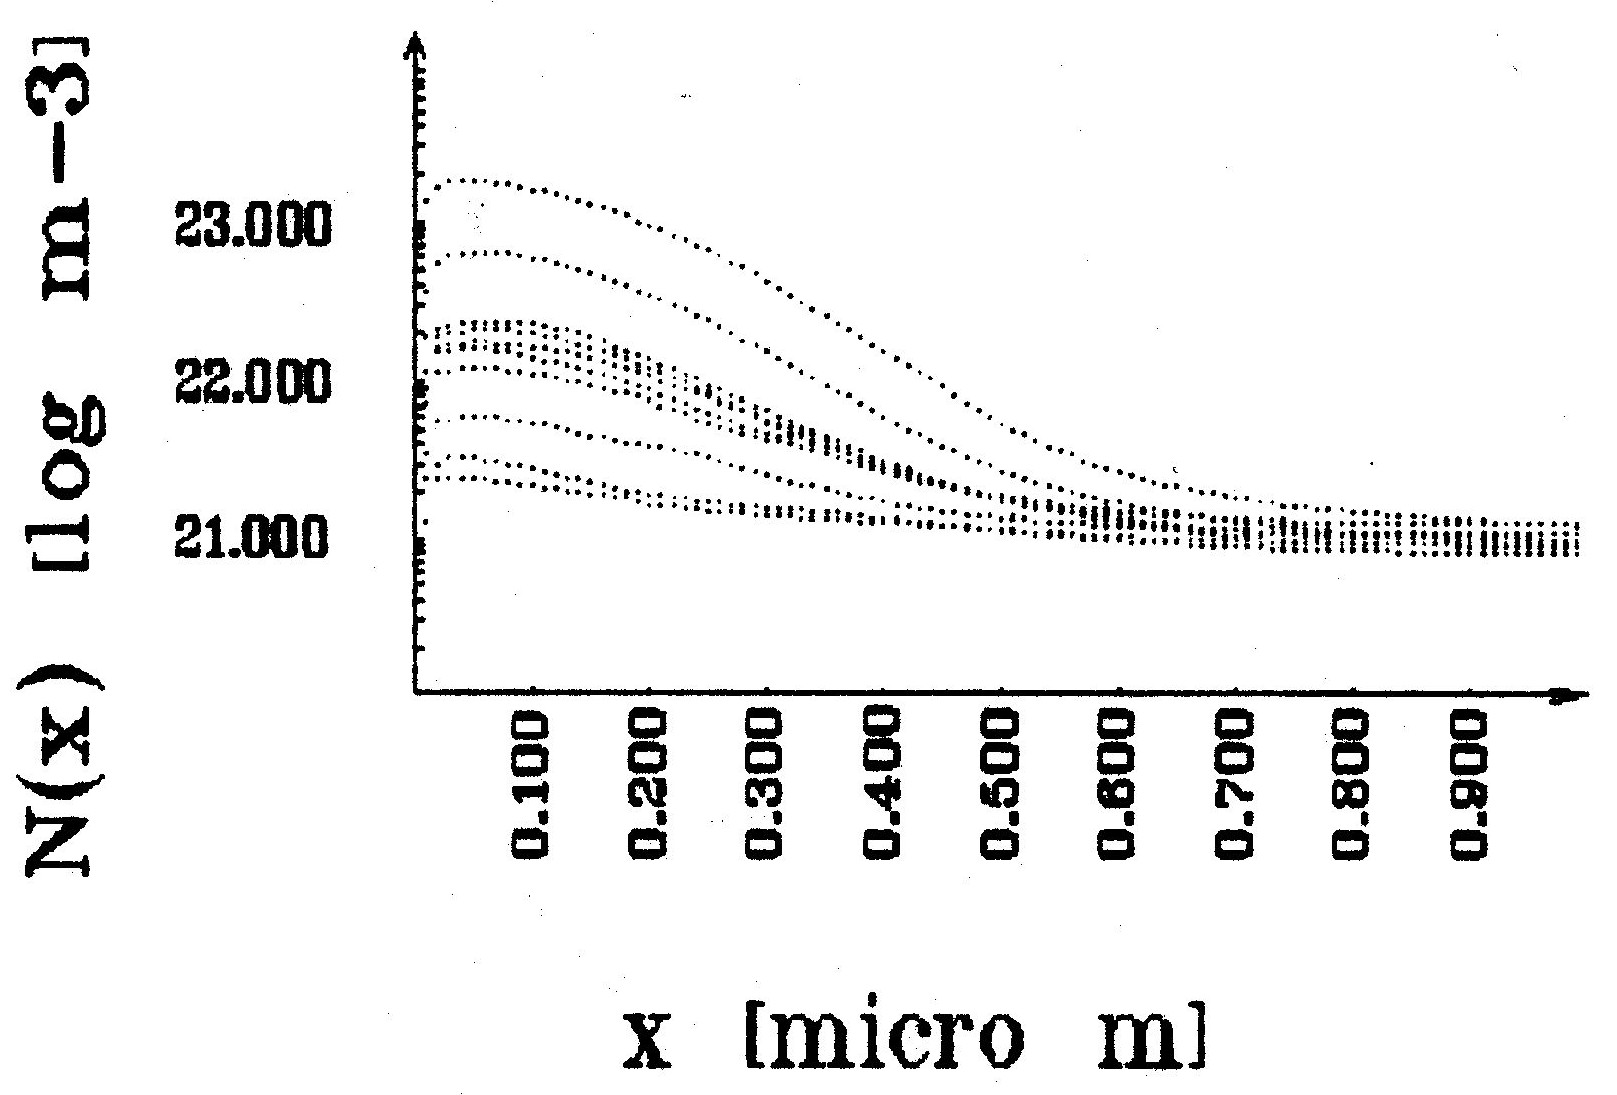
\includegraphics{Figures/fig-7-3.eps}
  \caption[Depth profile of tangents]{Depth profile of the interfering
    impurities in the subsurface region of the semiconductor formed by
    ion implantation with doses of $0.6, 1.0, 2.0, 4.0, 5.0, 6.0, 7.0,
    8.0, 20.0, 60.0 \times 10^{15} m^{-2}$. Shown are the $N(x)$
    waveforms represent the mean of the waveforms measured at 304 MOS
    structures of each silicon wafer.}\label{fig:7.3}
\end{figure}
% OBR27.BIT

\begin{table}[h!]\centering
  \begin{tabular}{c c c c}
    No. & ${D_{i}}{10}^{15}[m^{-2}]$ & $\overline{D}{10}^{15}[m^{-2}]$ & $\delta{D}{10}^{15}[m^{-2}]$\\
    \hline
    1 & 0.6 & 0.39 & 0.02\\
    3 & 1.0 & 0.59 & 0.08\\
    5 & 2.0 & 1.20 & 0.06\\
    7 & 4.0 & 2.67 & 0.09\\
    9 & 5.0 & 3.40 & 0.13\\
    11 & 6.0 & 4.07 & 0.13\\
    13 & 7.0 & 4.72 & 0.14\\
    15 & 8.0 & 5.49 & 0.09\\
    17 & 20.0 & 14.41 & 0.35\\
    19 & 60.0 & 42.63 & 0.21\\
  \end{tabular}
  \caption[Implantation dose $D_{i}$]{Implantation dose $D_{i}$, the
    calculated mean value of the implanted and activated ions in the
    semiconductor $\overline D$ and its standard deviation $\delta D$
    on the silicon wafer.}\label{tab:7.2}
\end{table}

Table~\ref{tab:7.2} contains the numerical values of the implant dose
entered during the implantation process $D_{i}$, the mean value of
$\overline D$ and the standard deviation of $\delta D$ of the doses
calculated by the procedure described in section~\ref{sec:6.1}.

To check the reproducibility of the implantation process, the
concentration profiles on 3 additional silicon wafers were
measured. In the Table~\ref{tab:7.3} are the implantation dose values
for the three pairs of silicon wafers that were implanted with the
same dose.

\newpage
\begin{figure}[h!]\centering
  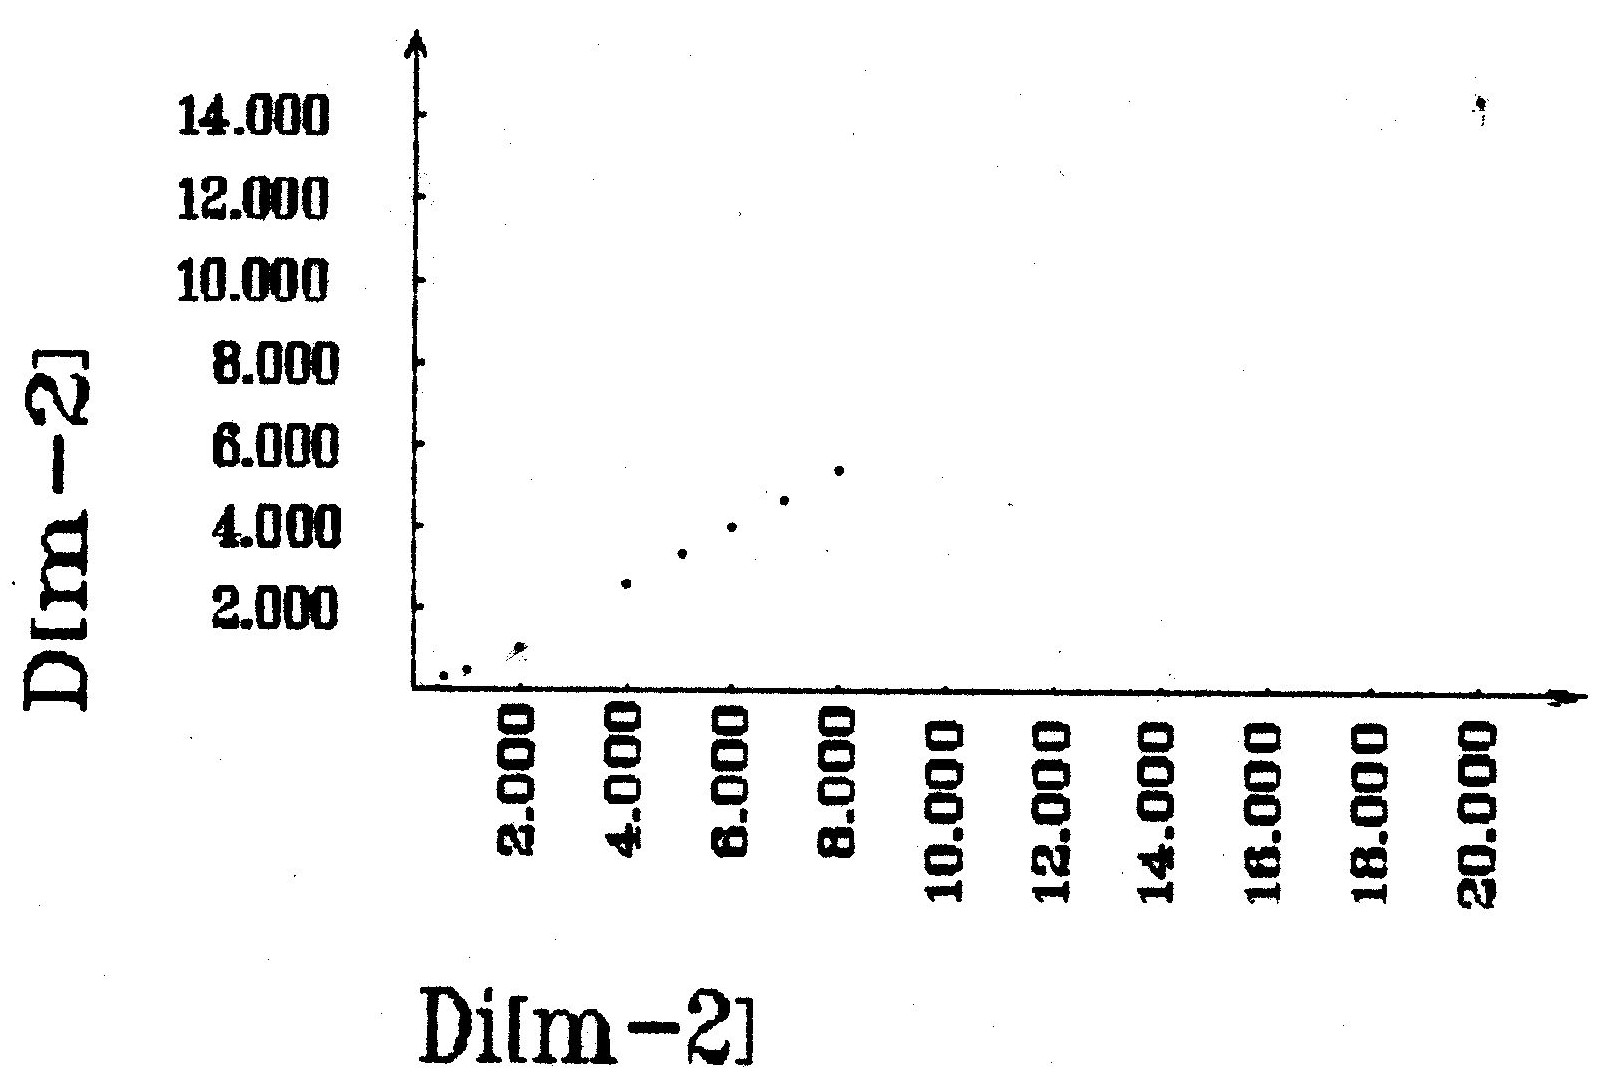
\includegraphics{Figures/fig-7-4.eps}
  \caption[Dependence of mean value
    $\overline{D}=E(\int(N(x)-N_{b})dx)$ on the implanted ion dose
    $D_{i}$]{Dependence of the mean value
    $\overline{D}=E(\int(N(x)-N_{b})dx)$ from the implanted ion dose
    $D_{i}$. Values shown are of order $10^{15}$.}\label{fig:7.4}
\end{figure}
%OBR29.BIT
 
\begin{table}[h!]\centering
  \begin{tabular}{c c c c}
    No. & $D_{i} 10^{15} [m^{-2}]$ & $\overline D 10^{15} [m^{-2}]$ & $\delta D 10^{15} [m^{-2}]$\\
    \hline
    9 & 5.0 & 3.40 & 0.13\\
    10 & 5.0 & 3.56 & 0.06\\
    11 & 6.0 & 4.07 & 0.13\\
    12 & 6.0 & 4.03 & 0.12\\
    15 & 8.0 & 5.49 & 0.09\\
    16 & 8.0 & 5.46 & 0.08\\
  \end{tabular}
  \caption[Implantation dose $D_{i}$]{Implantation dose $D_{i}$, the
    calculated mean of the dose of implanted and activated ions in the
    semiconductor $\overline D$ and its standard deviation $\delta D$
    on the silicon wafer.}\label{tab:7.3}
\end{table}

As can be seen from Table~\ref{tab:7.2} and~\ref{tab:7.3}, the
calculated implant dose is always less than the dose entered in the
process implantation. This is due, however, to the fact that the time
of implanted ions is trapped in the oxide layer, and yet incomplete
activation of the implanted ions in the semiconductor. In order to
determine the dependence between the specified and calculated dose, we
calculated by linear regression the coefficient $b$ of the relation

\begin{equation}\label{eq:7.1}
  \overline D = bD_{i}
\end{equation}

which had a value of $b = 0.71$ and we also plotted the dependence
$\overline D = f(D_{i})$ in Figure~\ref{fig:7.4}.

By doing so, we found that the original dose that was implanted became
electrically active $71\%$ of the implanted ions.

To determine the degree of dependence between the implanted dose and
the amount of electrically active impurities in the semiconductor,
which were implanted, we calculated the correlation coefficient
between these quantities. We used the relationship

\begin{equation}\label{eq:7.2}
  R(X,Y) = \frac{E([X-E(X)][Y-E(Y)])}{D(X)D(Y)}
\end{equation}

, which is given for example in~\cite{7.1}. In the
equation~\ref{eq:7.2} X and Y represent random variables, E represents
the mean and D denotes the standard deviation. This way we have
obtained the value of of the correlation coefficient

\centerline{$R(D_{i}, \overline{D}) = 0.99$}

taking the values of $D_{i}$ and $\overline{D}$ as realizations of the
random variable and we used all the values given in
Table~\ref{tab:7.2} and~\ref{tab:7.3}. It may be noted that in the
theory of probability the theorem is proved that $\rvert R(X,Y)\rvert
= 1$ precisely if, with probability 1, is valid

\centerline{$Y = a + b X$}

It follows that the dependence between the values of $D_{i}$ and
$\overline D$ is linear in this case.

\newpage
Using a professional program, purchased by Tesla Piešťany, to
simulate the process of ion implantation, the waveforms were
calculated of impurity concentration for doses of 0.6, 5.0 and 60.0
$\times10^{15}m^{-2}$.  The concentration profile waveforms were
simulated based on the specified implantation conditions using the
Pearson IV\@ method.  A comparison of the measured and simulated
impurity concentration waveforms is shown in Figure~\ref{fig:7.5}.

\begin{figure}[h!]\centering
  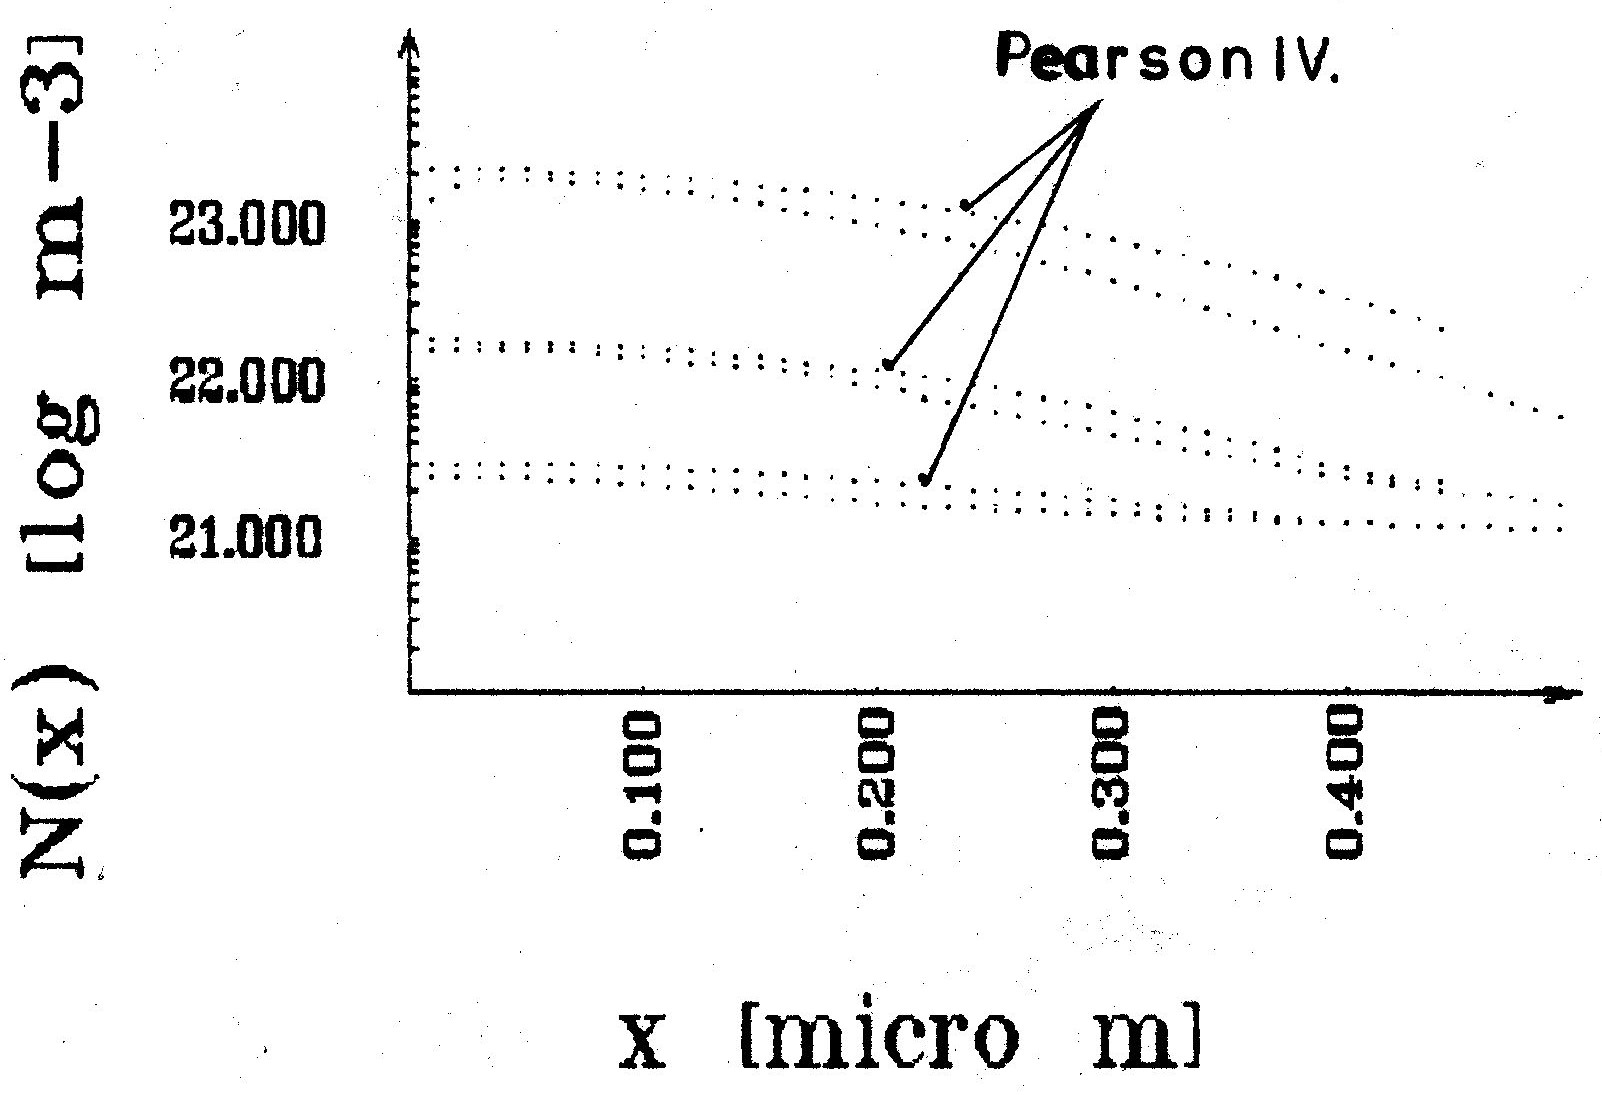
\includegraphics{Figures/fig-7-5.eps}
  \caption[Comparison of the mean values of the measured waveforms
    $N(x)$ and simulated using the Pearson IV method]{Comparison of
    means values of the measured $N(x)$ and simulated $N(x)$ waveforms
    Pearson IV for doses $0.6, 5.0, 60.0 \times 10^{15}
    m^{-2}$.}\label{fig:7.5}
\end{figure}
% OBR33.BIT

In the process of calculating the depth profiles of the intervening
admixtures, we simultaneously also determined the values of the
stresses of the aligned bands $V_{fb}$ for each MOS\@ structure
tested. Using a separate program that determines based on the data
contained in a given data file, the mean value and standard deviation
of the stored parameters, we calculated the mean of $\overline V{fb}$
and the standard deviation of $\delta V{fb}$. At the same time, using
the same procedure, we determined the values of $\overline h_{ox}$ and
$\delta h_{ox}$, which are for each silicon slabs are given in
Table~\ref{tab:7.4}.

It can be seen from the table~\ref{tab:7.4} that the values of
$\overline V_{fb}$ are related to the mean values of the oxide layer
thickness $\overline h_{ox}$, so we have shown this dependence in
Figure~\ref{fig:7.6}.

\newpage
\begin{figure}[h!]\centering
  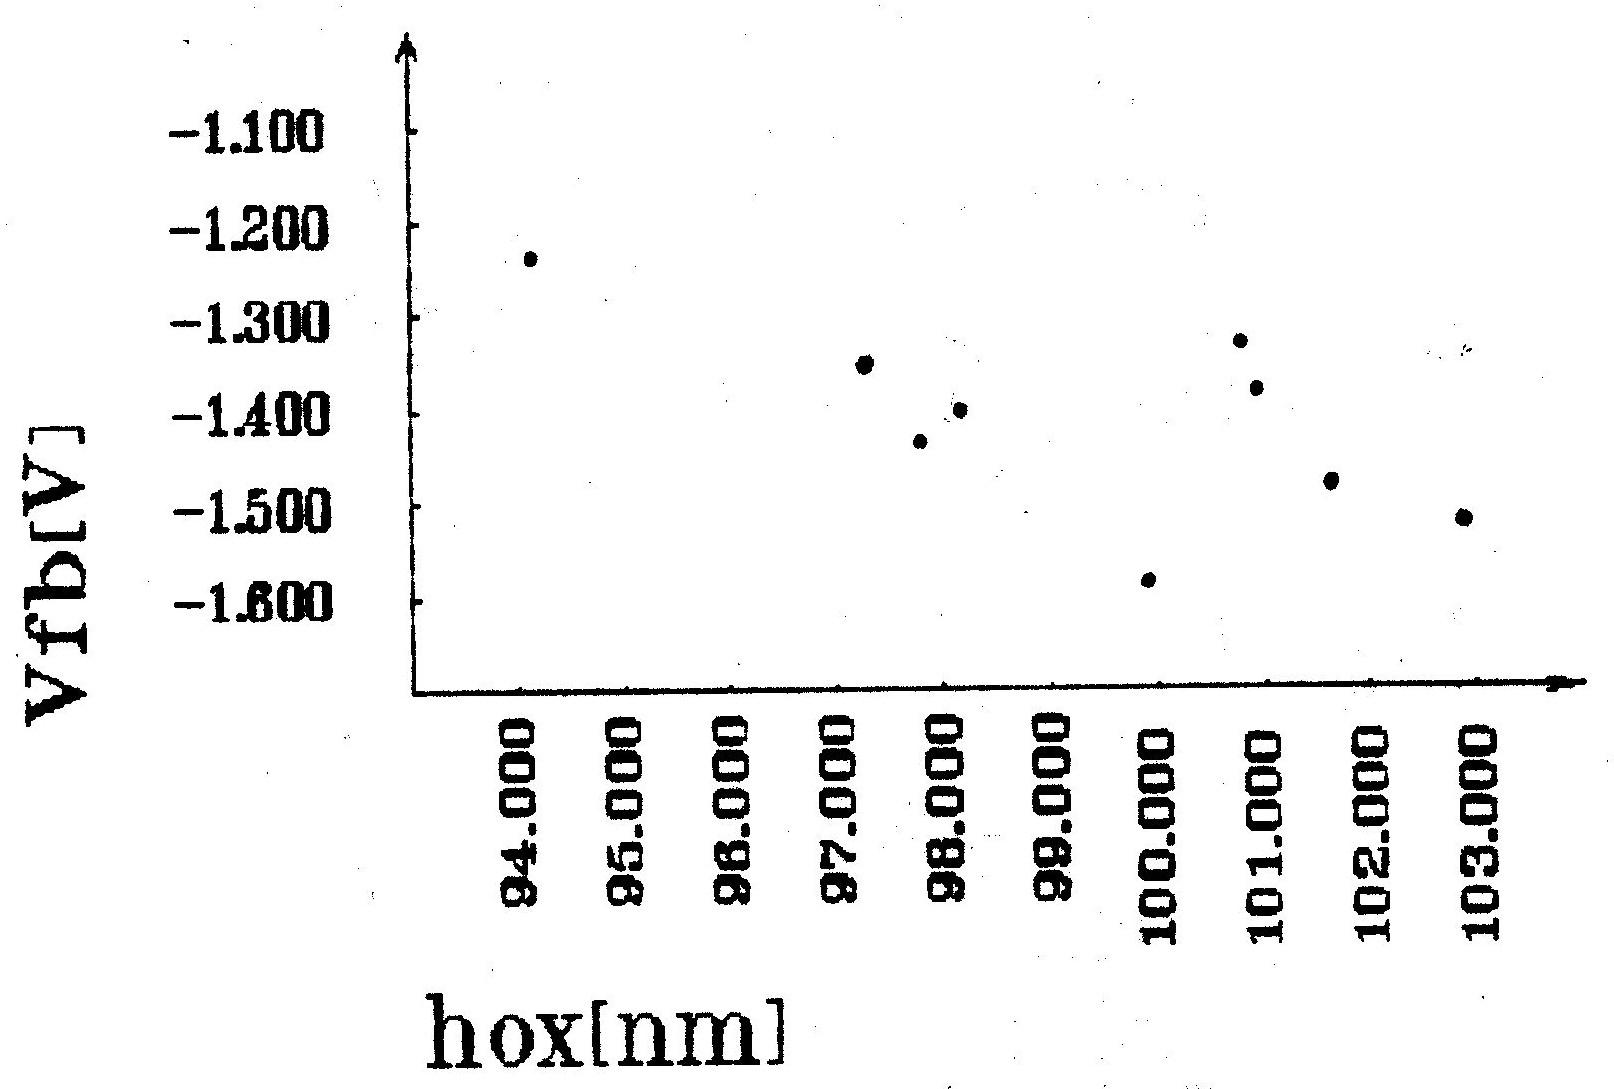
\includegraphics{Figures/fig-7-6.eps}
  \caption[Dependence of the mean value of $\overline V_{fb}$ on the
    mean value of the oxide layer thickness $\overline
    h_{ox}$]{Dependence of the mean value of $\overline V_{fb}$ on the
    mean value of the thickness of the oxide layer $\overline h_{ox}$
    for silicon wafers number 1, 3, 5, 7, 9, 11, 13, 15 and
    17.}\label{fig:7.6}
\end{figure}
% OBR28.BIT

\begin{table}[h!]\centering
  \begin{tabular}{c c c c c}
    No. & $\overline V_{fb} [V]$ & $\delta V_{fb} [V]$ & $\overline h_{ox} [nm]$ & $\delta h_{ox} [nm]$\\
    \hline
    1 & -1.24 & 0.07 & 94.14 & 0.89\\
    3 & -1.43 & 0.07 & 97.79 & 0.80\\
    5 & -1.35 & 0.08 & 97.26 & 0.28\\
    7 & -1.40 & 0.09 & 98.15 & 0.35\\
    9 & -1.52 & 0.09 & 102.85 & 0.53\\
    11 & -1.48 & 0.08 & 101.65 & 0.32\\
    13 & -1.38 & 0.08 & 100.94 & 0.41\\
    15 & -1.33 & 0.07 & 100.80 & 0.16\\
    17 & -1.59 & 0.08 & 99.93 & 0.22\\
    19 & -2.43 & 0.16 & 99.67 & 0.19\\
  \end{tabular}
  \caption[Mean and standard deviation of the voltage of the aligned
    strips and oxide thickness]{Mean and standard deviation of aligned
    strip stress and oxide thickness.}\label{tab:7.4}
\end{table}

Correlation coefficient value

\centerline{$R(\overline V_{fb} ,\overline h_{ox}) = -0.78$}

agrees with the theoretical relationship defining the dependence of
$V_{fb}$ on the magnitude of the breakdown charge in the oxide layer
and at the interface $Si-SiO_{2}$ $Q_{dc}$ and on the magnitude of the
oxide layer capacitance $C_{ox}$

\begin{equation}\label{eq:7.3}
  V_{fb}  = \varphi_{ms} + \frac{Q_{dc}}{C_{ox}}
\end{equation}

where $\varphi_{ms}$ represents the difference in output potentials
between the semiconductor and the metal.

For linear regression coefficients

\centerline{$V_{fb}  = a + b h_{ox}$}

we obtained the values

\centerline{$a = 5.48 \times 10^{-3} \qquad b = -1.41 \times 10^{7}$}

The interface trap density was determined on four silicon wafers
$Si-SiO_2$ $D_{it}$. As can be seen from Table~\ref{tab:7.5}, the mean
values of $\overline D_{it}$ are in the region of $2.0-5.0\times
10^{14}$, which speaks for the good quality of the $Si-SiO_{2}$
interface.

The crystal quality is indicated by the magnitude of the generation
time of the minority charge carriers. In order to compare the quality
of the crystal for individual slabs, we determined on each silicon
slab the area distribution of $³tau_{g}$ at depths ranging from $0.9$
to $1.3 m$. For all slabs we then determined the mean value of
$\overline\tau_{g}$ and the standard deviation of $\overline\tau_{g}$
deviation of $\delta\tau_{g}$, the values of which are given in
Table~\ref{tab:7.6}. The values of $\overline\tau_{g}$ range in
between $0.41\ and\ 2.25 ms$, indicating a high quality of the
substrate. At the same time, it can be seen from Table~\ref{tab:7.6}
that the values of $\overline \tau_{g}$ are randomly varying and
cannot be found dependence on the other previously mentioned
parameters.

\begin{table}[h!]\centering
  \begin{tabular}{c c c}
    No. & ${\bar{D_{it}}}[m^{-2}eV^{-1}]$ & $\delta D_{it}[m^{-2}eV^{-1}]$\\
    \hline
    3 & $4.42 \times 10^{14}$ & $0.25 \times 10^{14}$\\
    7 & $2.60 \times 10^{14}$ & $0.15 \times 10^{14}$\\
    9 & $2.74 \times 10^{14}$ & $0.15 \times 10^{14}$\\
    12 & $3.55 \times 10^{14}$ & $0.16 \times 10^{14}$\\
  \end{tabular}
  \caption[Mean and standard deviation of trap densities of the
    $Si-SiO_{2}$ interface at the center of the forbidden band.]{Mean
    value and standard deviation of the trap density of the
    $Si-SiO_{2}$ interface at the centre of the forbidden
    band.}\label{tab:7.5}
\end{table}

\begin{table}[h!]\centering
  \begin{tabular}{c c c}
    No. & ${\bar{\tau_{g}}}[ms]$ & $\delta\tau_{g}[ms]$\\
    \hline
    1 & 1.93 & 0.12\\
    3 & 1.48 & 0.09\\
    5 & 1.84 & 0.09\\
    7 & 1.67 & 0.10\\
    10 & 1.95 & 0.09\\
    12 & 0.41 & 0.02\\
    15 & 1.74 & 0.09\\
    17 & 2.25 & 0.14\\
  \end{tabular}
  \caption[Mean and standard deviation of generation time of life of
    minority carriers of charge]{Mean and standard deviation of the
    generational lifetime of minority carriers of
    charge.}\label{tab:7.6}
\end{table}


\begin{thebibliography}{}
\bibitem[7.1]{7.1}
  Renyi A.: Theory of Probability. Academia Prague 1972.
\end{thebibliography}
